%% REPLACE sXXXXXXX with your student number
\def\studentNumber{s2177402}


%% START of YOUR ANSWERS
%% Add answers to the questions below, by replacing the text inside the brackets {} for \youranswer{ "Text to be replaced with your answer." }. 
%
% Do not delete the commands for adding figures and tables. Instead fill in the missing values with your experiment results, and replace the images with your own respective figures.
%
% You can generally delete the placeholder text, such as for example the text "Question Figure 2 - Replace the images ..." 
%
% There are 19 TEXT QUESTIONS (a few of the short first ones have their answers added to both the Introduction and the Abstract). Replace the text inside the brackets of the command \youranswer with your answer to the question.
%
% There are also 3 "questions" to replace some placeholder FIGURES with your own, and 3 "questions" asking you to fill in the missing entries in the TABLES provided. 
%
% NOTE! that questions are ordered by the order of appearance of their answers in the text, and not by the order you should tackle them. Specifically, you cannot answer Questions 2, 3, and 4 before concluding all of the relevant experiments and analysis. Similarly, you should fill in the TABLES and FIGURES before discussing the results presented there. 
%
% NOTE! If for some reason you do not manage to produce results for some FIGURES and TABLES, then you can get partial marks by discussing your expectations of the results in the relevant TEXT QUESTIONS (for example Question 8 makes use of Table 1 and Figure 2).
%
% Please refer to the coursework specification for more details.


%% - - - - - - - - - - - - TEXT QUESTIONS - - - - - - - - - - - - 

%% Question 1:
\newcommand{\questionOne} {
\youranswer{Overfitting is making prediction too strict in order to produce consistent predictions in a particular data set, so that it can not predict data well on test sets or other data sets.}
}

%% Question 2:
\newcommand{\questionTwo} {
\youranswer{With the increase of the width and depth of the architecture, the generalization gap increases and the overfitting becomes more obvious.}
}

%% Question 3:
\newcommand{\questionThree} {
\youranswer{Question 3 - Summarise what your results show you about the effect of the tested approaches on overfitting and the performance of the trained model}
}

%% Question 4:
\newcommand{\questionFour} {
\youranswer{Question 4 - Give your overall conclusions}
}

%% Question 5:
\newcommand{\questionFive} {
\youranswer{Overfitting is a phenomenon that model has too good results on the training set and not so good results on the test set. For example with the progress of learning epochs, the accuracy rate decreases or does not increase like that on training set and generalization gap increases sharply especially on test set.}
}

%% Question 6:
\newcommand{\questionSix} {
\youranswer{Overfitting occurs for a number of reasons. First, the modeling sample set is incorrectly selected. For example, the number of sample sets is too small, leading to the sample data is not enough to represent the predetermined classification. Second, the noise contained in the sample set is too large, leading to the machine to regard part of the noise as valid data and thus interfere with the classification. Thirdly, the model has too many parameters and too much complexity (too much width and depth). In general, when the error rate of the model in the validation set is not significantly reduced or even increases with the number of learning rounds, or the generalization gap is extremely large, we can think that overfitting has occurred. From a practical point of view, the most important point is the classification accuracy, and when the classification accuracy on the test set no longer increases with that of the training set, it can be considered that there is an overfitting.}
}

%% Question 7:
\newcommand{\questionSeven} {
\youranswer{These two figures reflect the performance of classification accuracy and cross entropy errors in training set and verification set. As you can see from these two graphs, both of them are steadily rising or falling in the training set. However, in the validation set, after the vertex of the image curve (the point with slope 0), the two develop in reverse. The cross entropy error shows an upward trend around the 15th epoch, which can be considered as a sign of overfitting. But from a practical point of view, what we really care about is improving the classification accuracy on the validation data, so we think that the vertex of the classification accuracy curve on the validation set is the point where overfitting begins to dominate learning.}
}

%% Question 8:
\newcommand{\questionEight} {
\youranswer{From Table 1 and Figure 2, we can see that with the increase of model width, the accuracy rate of prediction increases continuously in the training set. But the results on the validation set were roughly the same (around 0.8). As the width of the model increases, the cross entropy error decreases in the training set, but the generalization gap increases (from 0.148 to 0.811).At the same time, around the 20th epoch, the models with width 64 and 128 appeared overfitting (the accuracy on validation set stops increasing and the errors in the validation set increased rather than decreased).}
}

%% Question 9:
\newcommand{\questionNine} {
\youranswer{From the images and data, it can be seen that the model with width 32 is underfitting (the result on the verification set is much lower than the result on the training set), the model with width 64 and 128 is overfitting, and the model with width 128 is overfitting more seriously.
To some extent, this confirms the previous explanation of the cause of overfitting and the possibility of overfitting is higher when the model complexity is too high.}
}

%% Question 10:
\newcommand{\questionTen} {
<<<<<<< Updated upstream
\youranswer{Question 10 - Explain your network depth experiment results by using the relevant figure and table}
=======
\youranswer{On the training set, the classification accuracy becomes higher and the errors become lower as the depth of the model increases. However, in the validation set, the classification accuracy of the three models is roughly the same (only slightly improved with the increase of depth), and the error and generalization gaps become larger with the increase of depth.}
>>>>>>> Stashed changes
}

%% Question 11:
\newcommand{\questionEleven} {
<<<<<<< Updated upstream
\youranswer{Question 11 - Discuss whether varying depth affects the results in a consistent way, and whether the results are expected and match well with the prior knowledge (by which we mean your expectations as are formed from the relevant Theory and literature)}
=======
\youranswer{The effects of different depths on the results are consistent. As the depth of the model increases, the classification accuracy becomes higher in both sets, even if it is very small in the validation set. On the validation set, error and generalization gaps become larger with increasing depth.
This is consistent with the previous description of over-complex models leading to overfitting. As can be seen from the generalization gap, the overfitting of the model becomes more serious with the increase of depth.}
>>>>>>> Stashed changes
}

%% Question 12:
\newcommand{\questionTwelve} {
<<<<<<< Updated upstream
\youranswer{Question 12 - Compare and discuss how varying width and height changes the performance and overfitting in your experiments}
=======
\youranswer{With the increase of model complexity (width and depth), the performance of the model increases little, but the degree of overfitting increases significantly.}
>>>>>>> Stashed changes
}

%% Question 13:
\newcommand{\questionThirteen} {
<<<<<<< Updated upstream
\youranswer{Question 13 - Explain L1/L2 weight penalties first in words and then with formulas. Explain how they are incorporated to training and what hyperparameter(s) they require}
=======
\youranswer{In machine learning, the loss function is usually followed by an extra term. There are two common extra terms, L1-norm and L2-norm.
These two can be viewed as the penalty terms of the loss function.
L1-norm refers to the sum of the absolute values of each element in the weight vector W, usually expressed as \begin{equation}
\| \boldsymbol{v} \|_1 = \sum_{d=1}^D \left| v_d \right|,
\end{equation}}
>>>>>>> Stashed changes
}

%% Question 14:
\newcommand{\questionFourteen} {
\youranswer{Question 14 - Discuss how/why the weight penalties may address overfitting, discuss how L1 and L2 regularization differ and support your claims with references where possible}
}

%% Question 15:
\newcommand{\questionFifteen} {
\youranswer{Question 15 - Explain the experimental details (e.g. hyperparameters), discuss the results in terms of their generalization performance and overfitting}
}

%% Question 16:
\newcommand{\questionSixteen} {
\youranswer{Question 16 - Explain the motivation behind Maxout Networks as presented in \cite{goodfellow2013maxout}}
}

%% Question 17:
\newcommand{\questionSeventeen} {
\youranswer{Question 17 - State whether Dropout is compatible (can be used together) with Maxout and explain why}
}

%% Question 18:
\newcommand{\questionEighteen} {
\youranswer{Question 18 - Give an overview of the experiment setup in \cite{goodfellow2013maxout} and analyse it from the point of view of how convincing their conclusions are}
}

%% Question 19:
\newcommand{\questionNineteen} {
\youranswer{Question 19 - Briefly draw your conclusions based on the results from the previous sections (what are the take-away messages?) and conclude your report with a recommendation for future directions}
}


%% - - - - - - - - - - - - FIGURES - - - - - - - - - - - - 

%% Question Figure 2:
\newcommand{\questionFigureTwo} {
\youranswer{Question Figure 2 - Replace the images in Figure 2 with figures depicting the accuracy and error, training and validation curves for your experiments varying the number of hidden units.
%
\begin{figure}[t]
    \centering
    \begin{subfigure}{\linewidth}
        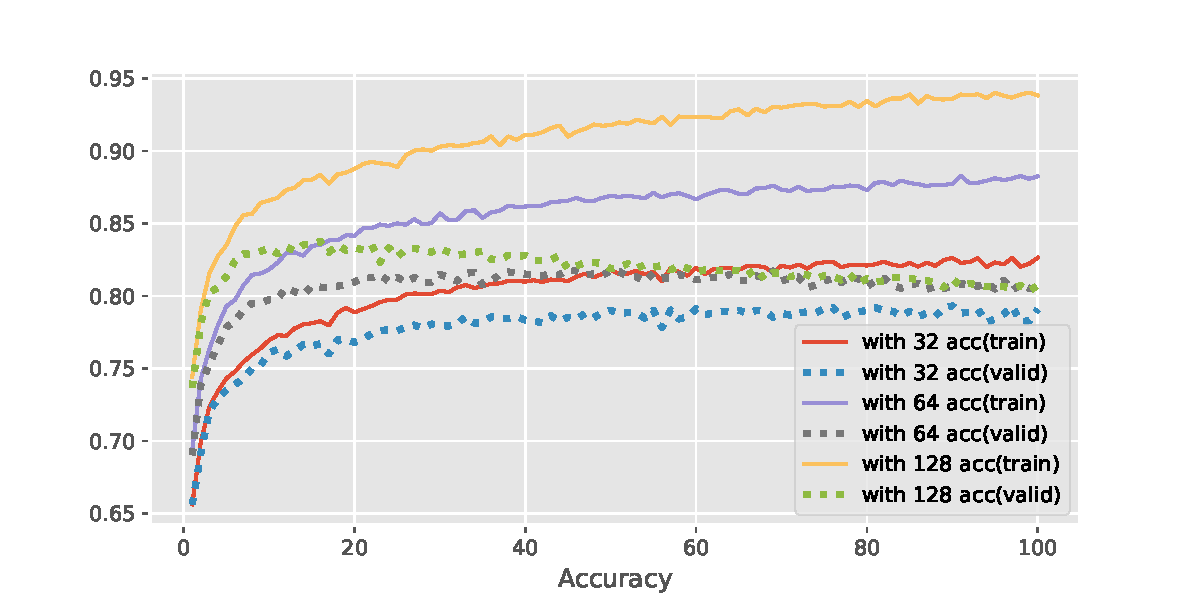
\includegraphics[width=\linewidth]{figures/empty_acc_curve_width_1.pdf}
        \caption{accuracy by epoch}
        \label{fig:width_acccurves}
    \end{subfigure} 
    \begin{subfigure}{\linewidth}
        \centering
        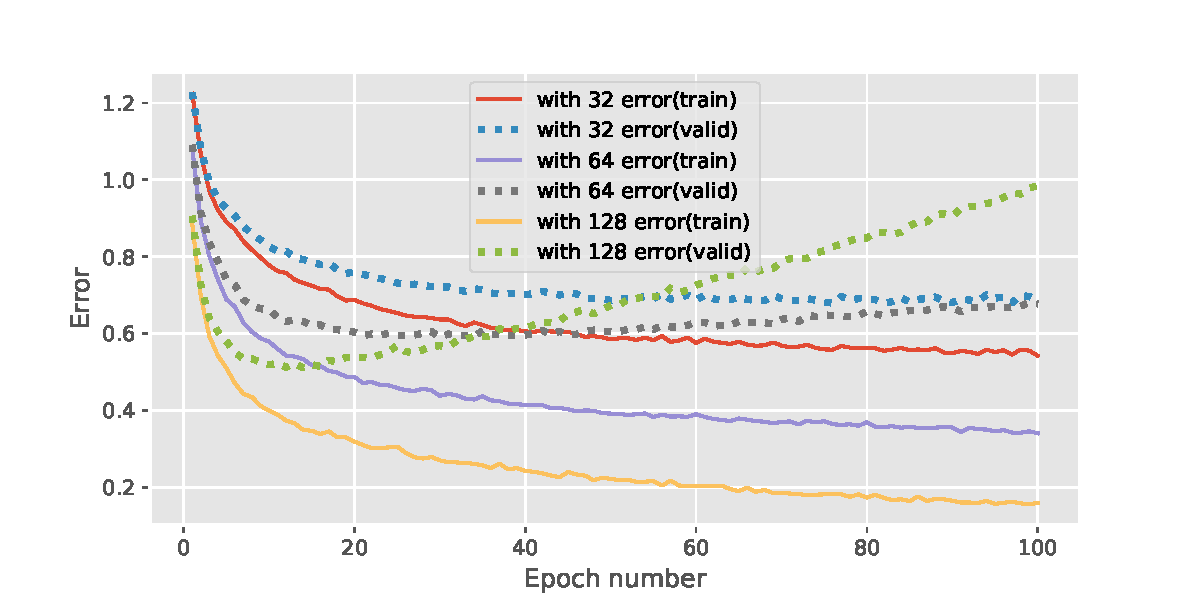
\includegraphics[width=\linewidth]{figures/empty_error_curve_width_1.pdf}
        \caption{error by epoch}
        \label{fig:width_errorcurves}
    \end{subfigure} 
    \caption{Training and validation curves in terms of classification accuracy (a) and cross-entropy error (b) on the EMNIST dataset for different network widths.}
    \label{fig:width}
\end{figure} 
}
}

%% Question Figure 3:
\newcommand{\questionFigureThree} {
\youranswer{Question Figure 3 - Replace these images with figures depicting the accuracy and error, training and validation curves for your experiments varying the number of hidden layers.
%
\begin{figure}[t]
    \centering
    \begin{subfigure}{\linewidth}
        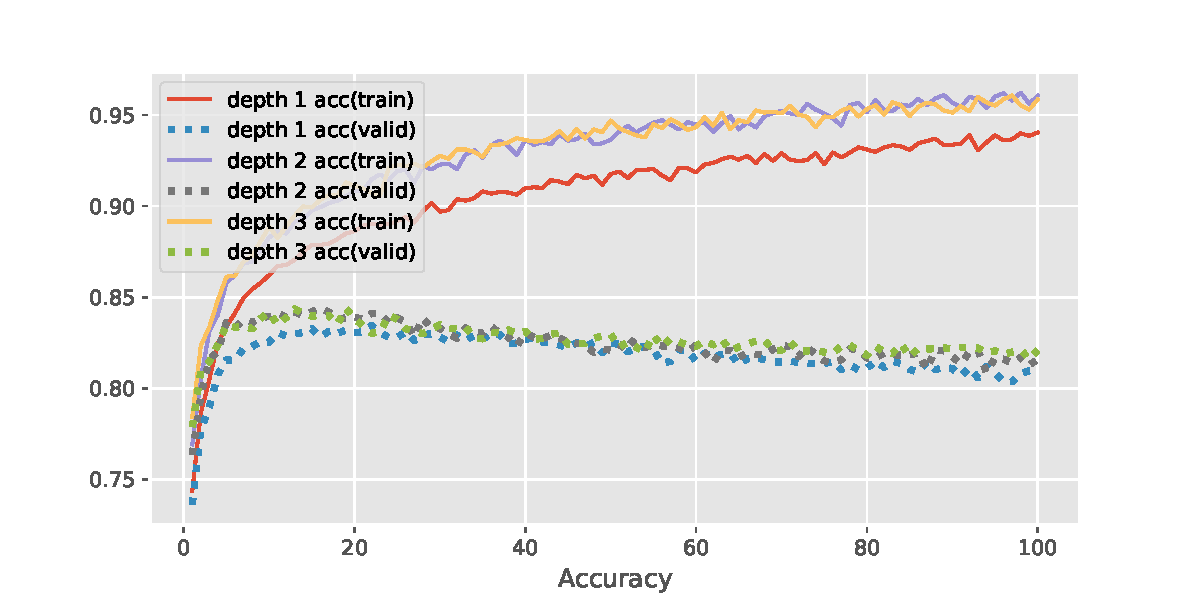
\includegraphics[width=\linewidth]{figures/empty_acc_curve_depth_1.pdf}
        \caption{accuracy by epoch}
        \label{fig:depth_acccurves}
    \end{subfigure} 
    \begin{subfigure}{\linewidth}
        \centering
        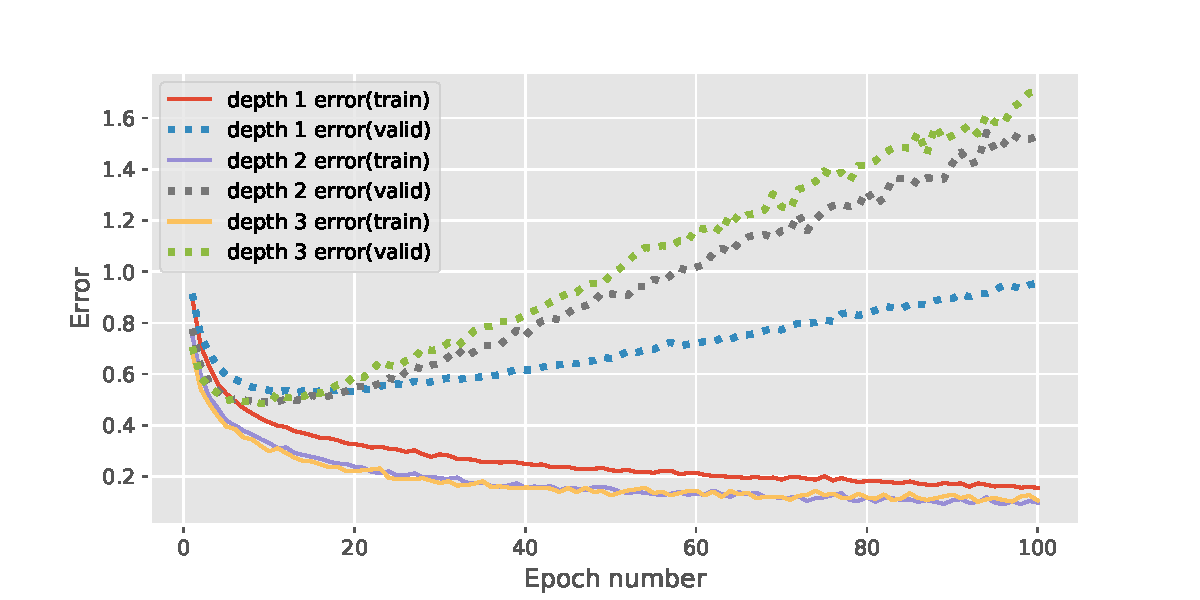
\includegraphics[width=\linewidth]{figures/empty_error_curve_depth_1.pdf}
        \caption{error by epoch}
        \label{fig:depth_errorcurves}
    \end{subfigure} 
    \caption{Training and validation curves in terms of classification accuracy (a) and cross-entropy error (b) on the EMNIST dataset for different network depths.}
    \label{fig:depth}
\end{figure} 
}
}

%% Question Figure 4:
\newcommand{\questionFigureFour} {
\youranswer{Question Figure 4 - Replace these images with figures depicting the Validation Accuracy and Generalisation Gap for each of your experiments varying the Dropout inclusion rate, L1/L2 weight penalty, and for the 8 combined experiments (you will have to find a way to best display this information in one subfigure).
%
\begin{figure*}[t]
    \centering
    \begin{subfigure}{.3\linewidth}
        \includegraphics[width=\linewidth]{figures/empty_dropout_plot.png}
        \caption{Metrics by inclusion rate}
        \label{fig:dropoutrates}
    \end{subfigure} 
    \begin{subfigure}{.3\linewidth}
        \centering
        \includegraphics[width=\linewidth]{figures/empty_wd_plot.png}
        \caption{Metrics by weight penalty}
        \label{fig:weightrates}
    \end{subfigure} 
    \begin{subfigure}{.3\linewidth}
        \centering
        \includegraphics[width=.85\linewidth]{example-image-duck}
        \caption{Extra experiments}
        \label{fig:extra}
    \end{subfigure} 
    \caption{Hyperparameter search for every method and combinations}
    \label{fig:hp_search}
\end{figure*}
}
}

%% - - - - - - - - - - - - TABLES - - - - - - - - - - - - 

%% Question Table 1:
\newcommand{\questionTableOne} {
\youranswer{
Question Table 1 - Fill in Table 1 with the results from your experiments varying the number of hidden units.
%
\begin{table}[t]
    \centering
    \begin{tabular}{c|cc}
    \toprule
        \# hidden units & val. acc. & generalization gap \\
    \midrule
         32            & 0.788           & 0.148                   \\
         64            & 0.805           & 0.344                   \\
         128           & 0.807           & 0.811                   \\ 
    \bottomrule
    \end{tabular}
    \caption{Validation accuracy (\%) and generalization gap (in terms of cross-entropy error) for varying network widths on the EMNIST dataset.}
    \label{tab:width_exp}
\end{table}
}
}

%% Question Table 2:
\newcommand{\questionTableTwo} {
\youranswer{
Question Table 2 - Fill in Table 2 with the results from your experiments varying the number of hidden layers.
%
\begin{table}[t]
    \centering
    \begin{tabular}{c|cc}
    \toprule
        \# hidden layers & val. acc. & generalization gap \\
    \midrule
         1               & 0.809           & 0.800                   \\
         2               & 0.816           & 1.432                   \\
         3               & 0.821           & 1.594                   \\ 
    \bottomrule
    \end{tabular}
    \caption{Validation accuracy (\%) and generalization gap (in terms of cross-entropy error) for varying network depths on the EMNIST dataset.}
    \label{tab:depth_exps}
\end{table}
}
}

%% Question Table 3:
\newcommand{\questionTableThree} {
\youranswer{
Question Table 3 - Fill in Table 3 with the results from your experiments varying the hyperparameter values for each of L1 regularisation, L2 regularisation, and Dropout (use the values shown on the table) as well as the results for your experiments combining L1/L2 and Dropout (you will have to pick what combinations of hyperparameter values to test for the combined experiments; each of the combined experiments will need to use Dropout and either L1 or L2 regularisation; run an experiment for each of 8 different combinations). Use \textit{italics} to print the best result per criterion for each set of experiments, and \textbf{bold} for the overall best result per criterion.
%
\begin{table*}[t]
    \centering
    \begin{tabular}{c|c|cc}
    \toprule
        Model    &  Hyperparameter value(s) & Validation accuracy & Generalization gap \\
    \midrule
    \midrule
        Baseline &  -                    &               0.836 &                 0.290 \\
    \midrule
        \multirow{3}*{Dropout}
                 & 0.7                   &                     &                   \\
                 & 0.9                   &                     &                   \\
                 & 0.95                  &                     &                   \\
    \midrule
        \multirow{3}*{L1 penalty}
                 & 1e-4                   &                     &                   \\
                 & 1e-3                   &                     &                   \\
                 & 1e-1                   &                     &                   \\
    \midrule
        \multirow{3}*{L2 penalty}  
                 & 1e-4                   &                     &                   \\
                 & 1e-3                   &                     &                   \\
                 & 1e-1                   &                     &                   \\
    \midrule
        \multirow{6}*{Combined}  
                 & for example 0.95, L1 1e-6  &                     &                   \\
                 & ?, ?                   &                     &                   \\
                 & ?, ?                   &                     &                   \\
                 & ?, ?                   &                     &                   \\
                 & ?, ?                   &                     &                   \\
                 & ?, ?                   &                     &                   \\
    \bottomrule
    \end{tabular}
    \caption{Results of all hyperparameter search experiments. \emph{italics} indicate the best results per series and \textbf{bold} indicate the best overall}
    \label{tab:hp_search}
\end{table*}
}
}

%% END of YOUR ANSWERS